%\documentclass[aps,pra,showpacs,notitlepage,onecolumn,superscriptaddress,nofootinbib,preprintnumbers]{revtex4-1}

%%%---TO DO------
% Discuss extentions to non-gaussians
% Use of ChatGPT
% Riordan-Touchard formula
% Proof structure, cavity connections. References for cavity method
% Open questions quantum spin glasses. Limit existence. Sequential version on lattices. Matching our and physics answers analytically



\newcommand{\fran}[1]{{\color{red}\small [Fran: #1]}}


\documentclass[12pt]{article}
%\documentclass{sig-alternate}


\usepackage{subfigure}



 \usepackage[utf8]{inputenc}
  \usepackage[noTeX]{mmap}
  \usepackage[T1]{fontenc}
\usepackage{authblk}

\usepackage{latexsym}
\usepackage{graphics}
\usepackage{amsmath}
\usepackage{xspace}
\usepackage{amssymb}
\usepackage{psfrag}
\usepackage{epsfig}
\usepackage{amsthm}
\usepackage{pst-all}
%\usepackage{auto-pst-pdf}
%\usepackage{hyperref}

\usepackage{color}

\definecolor{Red}{rgb}{1,0,0}
\definecolor{Blue}{rgb}{0,0,1}
\definecolor{Olive}{rgb}{0.41,0.55,0.13}
\definecolor{Yarok}{rgb}{0,0.5,0}
\definecolor{Green}{rgb}{0,1,0}
\definecolor{MGreen}{rgb}{0,0.8,0}
\definecolor{DGreen}{rgb}{0,0.55,0}
\definecolor{Yellow}{rgb}{1,1,0}
\definecolor{Cyan}{rgb}{0,1,1}
\definecolor{Magenta}{rgb}{1,0,1}
\definecolor{Orange}{rgb}{1,.5,0}
\definecolor{Violet}{rgb}{.5,0,.5}
\definecolor{Purple}{rgb}{.75,0,.25}
\definecolor{Brown}{rgb}{.75,.5,.25}
\definecolor{Grey}{rgb}{.5,.5,.5}

\def\red{\color{Red}}
\def\blue{\color{Blue}}
\def\yarok{\color{Yarok}}
%\def\olive{\color{Olive}}
%\def\green{\color{Green}}
%\def\mgreen{\color{MGreen}}
\def\dgreen{\color{DGreen}}
%\def\yellow{\color{Yellow}}
%\def\cyan{\color{Cyan}}
%\def\magenta{\color{Magenta}}
%\def\orange{\color{Orange}}
%\def\violet{\color{Violet}}
%\def\purple{\color{Purple}}
%\def\brown{\color{Brown}}
%\def\grey{\color{Grey}}

%\newcommand{\mnote}[1]{{\red Madhu's Note: #1}}
%\newcommand{\dnote}[1]{{\dgreen David's Note: #1}}

\newcommand{\bfX}{{\bf X}}
\newcommand{\bfU}{{\bf U}}
\newcommand{\bfu}{{\bf u}}
\newcommand{\bfV}{{\bf V}}
\newcommand{\bfv}{{\bf v}}
\newcommand{\bfT}{{\bf T}}
\newcommand{\bfx}{\mbox{\bf x}}
\newcommand{\bfY}{{\bf Y}}
\newcommand{\bfZ}{{\bf Z}}
\newcommand{\bfz}{{\bf z}}
\newcommand{\bfPhi}{{\bf\Phi}}


\setlength{\oddsidemargin}{-.20in}
\setlength{\evensidemargin}{-.20in} \setlength{\textwidth}{6.8in}
\setlength{\topmargin}{-0.6in} \setlength{\textheight}{9.1in}

\pagenumbering{arabic}


\newcommand{\Pois}{\ensuremath{\operatorname{Pois}}\xspace}
\newcommand{\Exp}{\ensuremath{\operatorname{Exp}}\xspace}
\newcommand{\Bi}{\ensuremath{\operatorname{Bi}}\xspace}
\newcommand{\Be}{\ensuremath{\operatorname{Be}}\xspace}
\newcommand{\Perm}{\ensuremath{\operatorname{Perm}}\xspace}
\newcommand{\Hom}{\ensuremath{\operatorname{Hom}}\xspace}
%\newcommand{\Trace}{\ensuremath{\operatorname{Tr}}\xspace}
%\newcommand{\hom}{\ensuremath{\operatorname{hom}}\xspace}

\def\smskip{\par\vskip 7pt}
\newcommand{\vvert}{\vspace{.1in}}
\newcommand{\pr}{\mathbb{P}}
%\newcommand{\E}{\mathbb{E}}
%\newcommand{\E}[1]{\mathbb{E}\!\left[#1\right]}
%\newcommand{\R}{\mathbb{R}}
%\newcommand{\Z}{\mathbb{Z}}
\newcommand{\N}{\mathbb{N}}
%\newcommand{\C}{\mathbb{C}}
\newcommand{\G}{\mathbb{G}}
%\newcommand{\F}{\mathbb{F}}
\newcommand{\Hg}{\mathbb{H}}
\newcommand{\HH}{\mathcal{H}}
\newcommand{\T}{\mathbb{T}}
\newcommand{\Lnorm}{\mathbb{L}}
\newcommand{\distr}{\stackrel{d}{=}}

\newcommand{\bincube}{\{0,1\}^{n\choose 2}}



\newcommand{\I}{{\bf \mathcal{I}}}
\newcommand{\M}{{\bf \mathcal{M}}}
%\newcommand{\N}{{\bf \mathcal{N}}}
\newcommand{\Overlap}{\mathcal{\mathcal{O}}}
\newcommand{\ROverlap}{\mathcal{\mathcal{R}}}

\newcommand{\mb}[1]{\mbox{\boldmath $#1$}}
\newcommand{\mbp}{\mb{p}}
\newcommand{\mbx}{\mb{x}}
\newcommand{\mby}{\mb{y}}
\newcommand{\mbz}{\mb{z}}
\newcommand{\mbI}{\mb{I}}
\newcommand{\mbL}{\mb{L}}
\newcommand{\mbM}{\mb{M}}
\newcommand{\mbZ}{\mb{Z}}
\newcommand{\zero}{\mb{0}}
\newcommand{\alphal}{\underline{\alpha}}
\newcommand{\alphau}{\bar{\alpha}}
\newcommand{\q}{[q^-]}
\newcommand{\rM}{\mathcal{M}}
\newcommand{\Dk}{[0,D]^{(k+1)\times k}}
\newcommand{\Dm}{[0,D]^{(m+1)\times m}}
\newcommand{\tomega}{\tilde{\omega}}

\newcommand{\calD}{{\cal D}}
\newcommand{\calG}{{\cal G}}
\newcommand{\sign}{\mathrm{sign}}


\newcommand{\ignore}[1]{\relax}

\newcommand{\even}{\text{even}}
\newcommand{\odd}{\text{odd}}


\newcommand{\ER}{Erd{\"o}s-R\'{e}nyi }
\newcommand{\Lovasz}{Lov\'{a}sz}
\newcommand{\local}{decimation}



%\newcommand{\dg}[1]{{\small \color{red}[David: #1]}}


%%---------------------------------- COLOR EDITTING ADDED BY MOHSEN --------------
%%--------------------------------------------------------------------------------
\definecolor{Red}{rgb}{1,0,0}
\definecolor{Blue}{rgb}{0,0,1}
\definecolor{Olive}{rgb}{0.41,0.55,0.13}
\definecolor{Green}{rgb}{0,1,0}
\definecolor{MGreen}{rgb}{0,0.8,0}
\definecolor{DGreen}{rgb}{0,0.55,0}
\definecolor{Yellow}{rgb}{1,1,0}
\definecolor{Cyan}{rgb}{0,1,1}
\definecolor{Magenta}{rgb}{1,0,1}
\definecolor{Orange}{rgb}{1,.5,0}
\definecolor{Violet}{rgb}{.5,0,.5}
\definecolor{Purple}{rgb}{.75,0,.25}
\definecolor{Brown}{rgb}{.75,.5,.25}
\definecolor{Grey}{rgb}{.5,.5,.5}
\definecolor{Pink}{rgb}{1,0,1}
\definecolor{DBrown}{rgb}{.5,.34,.16}
\definecolor{Black}{rgb}{0,0,0}

\def\red{\color{Red}}
\def\blue{\color{Blue}}
\def\olive{\color{Olive}}
\def\green{\color{Green}}
\def\mgreen{\color{MGreen}}
\def\dgreen{\color{DGreen}}
\def\yellow{\color{Yellow}}
\def\cyan{\color{Cyan}}
\def\magenta{\color{Magenta}}
\def\orange{\color{Orange}}
\def\violet{\color{Violet}}
\def\purple{\color{Purple}}
\def\brown{\color{Brown}}
\def\grey{\color{Grey}}
\def\doubt{\color{Pink}}
\def\dbrown{\color{DBrown}}
\def\black{\color{Black}}

%%------------------------------------------------------
%% How to remove colors
\long\def\mnew#1{{\blue #1}}   %%  Use this to add colors

%\long\def\mnew#1{{#1}}   %%  Use this to remove the colors


%%------------------------------------------------------






%%%%%%%%%---------

\usepackage{bbm}
\usepackage{mathrsfs}
\usepackage{epsfig}
\usepackage{soul,color}
\usepackage{graphicx}
\usepackage{amsfonts}
\usepackage{amsthm}
\usepackage[figuresright]{rotating}
\usepackage{amssymb}
\usepackage{amsmath}
\usepackage{dcolumn}
\usepackage{physics}
\usepackage{float}
\usepackage{bm}
\usepackage{verbatim}
\usepackage[normalem]{ulem}
\usepackage[colorlinks,linkcolor=blue,anchorcolor=blue,citecolor=blue,urlcolor=blue]{hyperref}
\usepackage{mathtools}

\usepackage{algorithm}
\usepackage{algorithmic}

\usepackage{xcolor}
\newtheorem{theorem}{Theorem}
\newtheorem{lemma}[theorem]{Lemma}
\newtheorem{conjecture}[theorem]{Conjecture}
\newtheorem{proposition}[theorem]{Proposition}
\newtheorem{corollary}[theorem]{Corollary}
\newtheorem{definition}{Definition}[section]
\newtheorem{assumption}{Assumption}[section]
\newtheorem{fact}{Fact}[section]
\newtheorem{example}{Example}[section]
\newtheorem{remark}{Remark}[section]

\renewcommand{\arraystretch}{1.2}

\newcommand{\plog}[1]{\mathrm{polylog}\left(#1\right)}
\newcommand{\poly}[1]{\mathrm{poly}\left(#1\right)}
%\newcommand{\pr}[1]{\mathrm{Pr}\left[#1\right]}
%\newcommand{\prr}[2]{\mathrm{Pr}_{#1}\left[#2\right]}
\newcommand{\lr}[1]{\left(#1\right)}
\newcommand{\EE}[1]{\mathbb{E}\left[#1\right]}
\newcommand{\E}{\mathbb{E}}
\newcommand{\Var}[1]{\mathrm{Var}\left[#1\right]}
\newcommand{\C}{\mathbb{C}}
\newcommand{\D}{\mathbb{D}}
\newcommand{\F}{\mathbb{F}}
\newcommand{\R}{\mathbb{R}}
\newcommand{\Z}{\mathbb{Z}}
\newcommand{\cA}{\mathcal{A}}
\newcommand{\cB}{\mathcal{B}}
\newcommand{\cC}{\mathcal{C}}
\newcommand{\cD}{\mathcal{D}}
\newcommand{\cE}{\mathcal{E}}
\newcommand{\cF}{\mathcal{F}}
\newcommand{\cG}{\mathcal{G}}
\newcommand{\cH}{\mathcal{H}}
\newcommand{\cJ}{\mathcal{J}}
\newcommand{\cK}{\mathcal{K}}
\newcommand{\cL}{\mathcal{L}}
\newcommand{\cM}{\mathcal{M}}
\newcommand{\cN}{\mathcal{N}}
\newcommand{\cO}{\mathcal{O}}
\newcommand{\cP}{\mathcal{P}}
\newcommand{\cR}{\mathcal{R}}
\newcommand{\cS}{\mathcal{S}}
\newcommand{\cT}{\mathcal{T}}
\newcommand{\cU}{\mathcal{U}}
\newcommand{\cV}{\mathcal{V}}
\newcommand{\cX}{\mathcal{X}}
\newcommand{\cZ}{\mathcal{Z}}
\newcommand{\wh}{\widehat}
\newcommand{\bin}{\mathrm{Binomial}}
\newcommand{\multi}{\mathrm{Multinomial}}
\newcommand{\bern}{\mathrm{Bernoulli}}
\newcommand{\poiss}{\mathrm{Poisson}}
\newcommand{\diag}{\mathrm{Diag}}
\newcommand{\supp}{\mathrm{supp}}
\newcommand{\Span}{\mathrm{span}}
\newcommand{\maxcut}{\textsf{MAX-CUT}}
\newcommand{\tot}{\mathrm{tot}}
\newcommand{\inter}{\mathrm{int}}
\newcommand{\bath}{\mathrm{bath}}
\newcommand{\pauli}{\mathrm{Pauli}}
\newcommand{\tv}{\mathrm{TV}}
\newcommand{\col}{\mathrm{Coll}}
\newcommand{\nocol}{\mathrm{NoColl}}
\newcommand{\DQC}{\mathrm{DQC1}}
\newcommand{\BPP}{\mathrm{BPP}}
\newcommand{\spec}{\mathrm{spec}}
\newcommand{\sep}{\mathrm{sep}}
\newcommand{\mix}{\mathrm{mix}}
\newcommand{\ann}{\mathrm{ann}}
\newcommand{\dist}{\mathrm{distinct}}
\newcommand{\rep}{\mathrm{rep}}
\newcommand{\conn}{\mathrm{conn}}
\newcommand{\id}{\mathbb{I}}
\newcommand{\crs}{\operatorname{cr}}





\newcommand{\dg}[1]{{\small \color{red}[David: #1]}}
\newcommand{\az}[1]{{\small \color{blue}[AZ: #1]}}


\begin{document}






\section*{Notations and conventions}
We close this section with some notational conventions. We let $[m]$ denote the set $\{1,2,\ldots,m\}$ for every positive integer $m$.
$\R,\C,\Z$ and $\Z_+$ stand for  the set of all real, complex, integer and non-negative integer values, respectively. 
$\Tr$ denotes the trace operator and $\tr=2^{-{n\over 2}}\Tr$ is the normalized trace (so that $\tr(\id)=1$ for the identity operator $\id$ in $\C^{2^{n\over 2}}$). 

Next we introduce some graph-theoretic notations.
A simple $q$-uniform hypergraph, or just simple hypergraph is a pair $(V,E)$ where $V$ is the set of nodes and $E$ is a  subset of the set of 
all ${V \choose q}$ cardinality $q$ subsets of $V$. 
For two hyperedges $e_1,e_2\in E$ we  write $e_1\sim e_2$ when $e_1\cap e_2\ne \emptyset$.
With some abuse of notation we let $\binom{V}{q}$ denote the set of all $q$-size subsets of $V$.
A multi $q$-uniform hypergraph, or just multi hypergraph, is a pair $(V,\bar r)$ where $\bar r\in \Z_+^{|V| \choose q}$. For each subset $e\in \binom{V}{q}$ 
$r_e\in \Z_+$ is called the multiplicity of the hyperedge $e$. $m(V,E)=\sum_{e\in \binom{V}{q}} r_e$ denotes the total multiplicity of the
multi hypergraph $(V,E)$.
Each multi hypergraph naturally induces a simple hypergraph where hyperedges are included
iff $r_e\ge 1$. Let $\cH^{\rm sim}([m])$ denote the set of all simple hypergraphs on the node set $[m]$. 
$\cH([m])$ denotes the  set of all multi hypergraphs on the node set $[m]$ with even  multiplicities, namely $r_e\in 2\Z_+$ for all $e$. 
Note that while $\cH^{\rm sim}([m])$ is a finite set for every $m$, the set $\cH([m])$ is infinite. 

A simple hypergraph $(V,E)$ is connected if for every $u,v\in V$ there exists a path from $u$ to $v$. Namely, there exists a sequence of hyperedges $e_1,\ldots,e_r$
such that $u\in e_1,v\in e_r$ and $e_i\cap e_{i+1}\ne\emptyset, i\in [r-1]$. A multi hypergraph is connected if its induced simple hypergraph is connected. 
Every simple and multi hypergraph $H$ admits a unique decomposition into 
connected components $H_1,\ldots,H_C$ so that $H$ is the disjoint union of $H_i$ and each $H_i$
is a connected hypergraph.
A simple hypergraph $(V,E)$ is  called a hypertree or simply a tree 
if it is a connected hypergraph with precisely $(|V|-1)/(q-1)$ hyperedges. 
It is easy to verify that every two hyperedges of a hypertree intersect in at most one node.
The set of all simple hypertrees 
on the node set $[m]$ is denoted by $\cT^{\rm sim}_m$. A singleton, namely a graph on one node with no hyperedges is defined to be connected by default, so that $\cT_{1}^{\rm sim}=\{1\}.$
A special role in our derivation 
will be played by multi hypertrees where all multiplicities are $r_e=2$, so that the total number of hyperedges is $2(m-1)/(q-1)$. We denote the set of
such hypertrees by $\cT_{m,2}$. Given $m\ge 1,\Delta\ge 0$, $\cH_{m,\Delta}\subset \cH([m])$ denotes the set of all connected multi hypergraphs  with 
precisely $2(m-1+\Delta)/(q-1)$ hyperedges. Note that $\cH_{v,0}=\cT_{v,2}$. We call $\Delta$ the excess of $H$ for $H\in\cH_{m,\Delta}$. 



\section{Main result. Free energy limit}
The  SYK model is defined on the Hilbert space  $\C^{2^{n\over 2}}$ via 
the so-called Majorana  operators $\psi_i, i\in [n]$ on $\C^{2^{n\over 2}}$ satisfying 
\begin{align}\label{eq:anti-commutation}
\{\psi_i, \psi_j\}\triangleq \psi_i\psi_j+\psi_j\psi_i=\delta_{ij}. 
\end{align}
Here $\delta_{ij}$ is the identity operator $\id$ on $\C^{2^{n\over 2}}$,  when $i=j$, and $0$ otherwise, 
so that $\psi_i^2={1\over 2}\id$. These operators can be explicitly constructed using standard Pauli 
operators $X,Y,Z$ by setting $\psi_{2i+1}={1\over \sqrt{2}}(\otimes_{1\le k\le i}Z) \otimes X_{i+1}\otimes \id$
and $\psi_{2i+2}={1\over \sqrt{2}}(\otimes_{1\le k\le i}Z) \otimes Y_{i+1}\otimes \id$, for $0\le i\le n/2-1$. 
This explicit construction though will not be necessary for us. We fix a positive even integer $q$, the interaction parameter. 
For every $I=(i_1,\ldots,i_q)\in \binom{[n]}{q}, 1\le i_1<\cdots<i_q \le n$ we define $ \psi_I \triangleq i^{q/2}\psi_{i_1}\cdots \psi_{i_q}$. In particular $\psi_I^2=2^{-q}\id$,
which is an easy implication of (\ref{eq:anti-commutation}).
The Hamiltonian of the SYK model with $q$-body interaction is then defined as
the Hermitian operator
\begin{align}\label{eq:H-definition}
    H_{\rm SYK} \triangleq \sum_{I \in \binom{[n]}{q}} J_I \psi_I,
\end{align}
where $(J_I, I\in \binom{[n]}{q})$ is a sequence of i.i.d. random variables defined by $J_I=\sigma \bar J_I$ where $\sigma^2 = \frac{(q-1)!}{n^{q-1}}$
and $\bar J_I$ are Rademacher random variables, independent across $I\in \binom{[n]}{q}$. 
I.e. $\bar J_I=\pm 1$ with equal probabilities $1/2$.
By the universality property established in~\cite{anschuetz2025bounds} 
the free energy limit (defined below) will be the same for the case when $\bar J_I$ are i.i.d. standard normal
random variables, which is a more common choice in defining the SYK Hamiltonian.
For every fixed inverse temperature $\beta\in\R$ we define the associated (random) partition function 
$Z_{n,q}(\beta) \triangleq \tr(e^{\beta H_{\rm SYK}})$, where we recall that $\tr=2^{-{n\over 2}}\Tr$ stands for the normalized trace operator.
The normalization by $2^{n\over 2}$ is chosen for convenience as the trace of the identity operator $\id$ in $\C^{2^{n\over 2}}$ is $2^{n\over 2}$.
 We define the associated free energy as
\begin{align*}
    F_{n,q}(\beta) \triangleq  {1\over \beta}\log Z_{n,q}(\beta). 
\end{align*}
Our main result is the computation of the free energy limit 
\begin{align*}
F_q(\beta)\triangleq \lim_{n\to \infty} {F_{n,q}(\beta) \over n},
\end{align*}
for small enough constant inverse temperature $\beta$. In particular, we  prove
 the existence of this limit (see the discussion in the introduction), and establish that it holds w.h.p. as $n\to\infty$.
In light of the ''quenched $\approx$ annealed'' result (\ref{eq:quenched-is-annealed}) mentioned earlier and in light of the 
concentration of the quenched free energy around its expectation, also verified  in~\cite{anschuetz2025bounds}, 
we instead focus on 
\begin{align*}
    f_{n,q}(\beta) \triangleq  {1\over \beta}\log \E[Z_{n,q}(\beta)].
\end{align*}
Thus our goal is proving  the existence and computing the limit 
\begin{align*}
f_q(\beta)\triangleq \lim_{n\to \infty} {f_{n,q}(\beta) \over n},
\end{align*}
as $f_q(\beta)=F_q(\beta)$ for all $\beta$.

In order to state our result formally, we begin by introducing some necessary  technical preliminaries. 
Let $\Omega=[0,1]^2$. Elements $x=(u_1,u_2)\in \Omega$ will be referred to as ''chords''.
For every  $x=(u_1,u_2), y=(v_1,v_2)\in \Omega$, define the chord intersection function
\begin{align*}
    K(x,y) = \begin{cases}
        -1 & \text{if}~u_1 < v_1 < u_2 < v_2 \text{ or } v_1 < u_1 < v_2 < u_2,\\
        1 & \mathrm{otherwise}.
    \end{cases}
\end{align*}
Namely $K(x,y)=-1$ when the chords $x$ and $y$ cross and $=1$ otherwise. Let $\nu$ be the probability law of $(\min(U_1,U_2),\max(U_1,U_2))\in\Omega$
when $U_j, j=1,2$ are generated uniformly at random from $[0,1]$, independently. 
\begin{figure}[H]
    \centering
    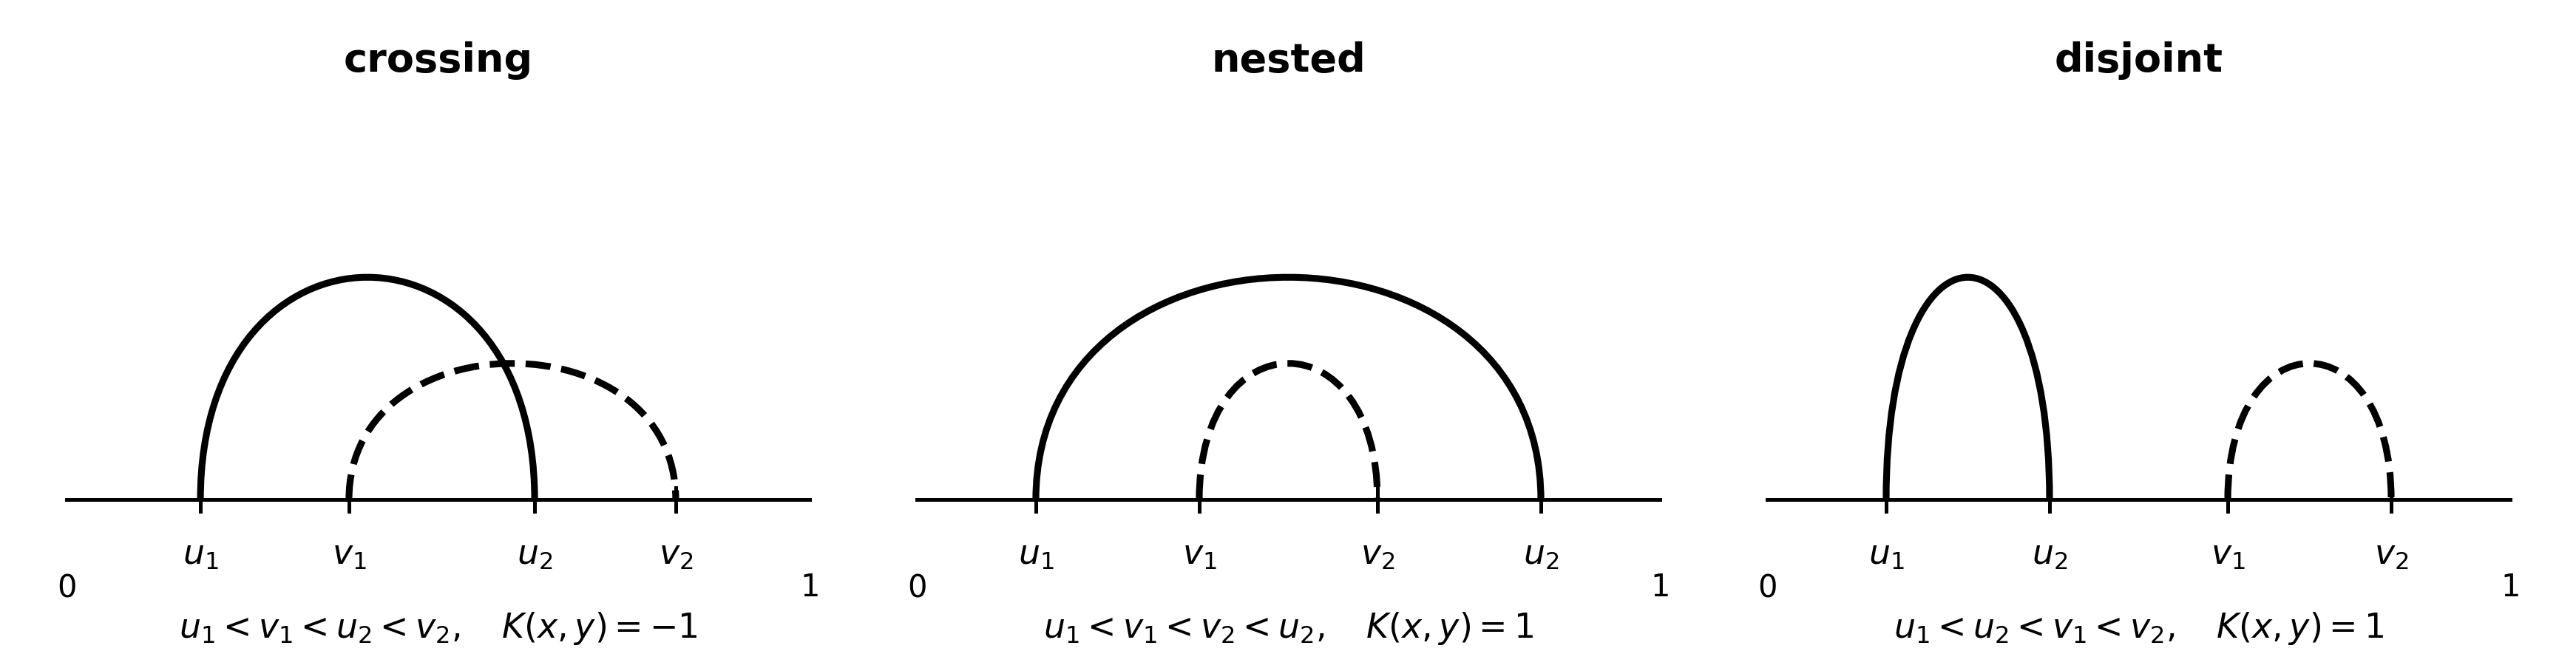
\includegraphics[width=\linewidth]{chord_intersection_figure_bw_v3.png}
    \caption{Chord intersection sign for two chords $x = (u_1,u_2),y=(v_1,v_2)\in \Omega.$}
    \label{fig:placeholder}
\end{figure}

On the space of continuous functions from $\{z\in \C: |z|\le 1/e^2\}\times \Omega$ to $\C$ 
define a norm $\|G\|_{e,\Omega}=\sup_{|z| \le 1/e^2, x\in\Omega} |G(z,x)|$. 
The restriction $|z|\le 1/e^2$ can be relaxed a little and is chosen for convenience.
Let $\mathcal{F}_{e,\Omega}$ 
be the subset of these functions $G$ satisfying $\|G\|_{e,\Omega}\le 1$.
On $\mathcal{F}_{e,\Omega}$ we introduce a function $H$, which 
we call the Chord-Cavity-Generator (CCG), defined implicitly via
the following fixed point equation
\begin{align}\label{eq:H-def}
 H(z,x)
        =
        z+ z\sum_{d\geq 1}\frac{1}{d!}
        \int_{\Omega^d}
        \prod_{i=1}^d
        \left[
            K(x,y_i)\,\frac{H(z,y_i)^{q-1}}{(q-1)!}
        \right]
        \prod_{1\leq i<j\leq d} K(y_i,y_j)\,
        \nu^{\otimes d}(dy_1\cdots dy_d).
\end{align}
The validity of this definition is justified by the following claim.
\begin{proposition}[Existence of CCG]\label{prop:existsCCG}
For every even $q\ge 2$ there exists $H\in\mathcal{F}_{e,\Omega}$ which is the unique solution of the equation (\ref{eq:H-def}). 
Furthermore, $H$ is analytic on the domain $\{z\in \C: |z|\le 1/e^2\}\times \Omega$.
\end{proposition}
The proof of this proposition is found in Section~\ref{section:loose-ends}.
Next we  provide a more intuitive and equivalent description of CCG via the chord crossing diagrams on trees. Consider any simple 
$q$-uniform hypergraph $H=(V,E)$ on the node set $V=V(H)$ and edge set $E=E(H)$.  
Suppose we have a chord mapping $X:E\to \Omega$. Define  
\begin{align*}
B_H(X)=\prod_{e_1,e_2\in E: |e_1\cap e_2|~{\rm odd}}K(X(e_1),X(e_2))\in \{\pm 1\}.
\end{align*}
Namely, $B_H(X)$ is $(-1)^R$, where $R$ is  the number of pairs of hyperedges which share an odd number of nodes and such that their corresponding chords cross. 
Let 
\begin{align}
b_H=\E[B_H(X)], \label{eq:b_H}
\end{align}
when $X$ is generated according to  the law $\nu^{\otimes |E|}$. Note that $| b_H|\le 1$.

Similarly, suppose we have a simple rooted hypergraph $H$ with a distinguished node $r\in V$ called a root. Fix $x\in \Omega$
and $X:E\to\Omega$. Define
\begin{align}
B_{H,r}(X,x)=\prod_{e\in E:r\in e}K(x,X(e)) 
\prod_{e_1,e_2\in E:|e_1\cap e_2|~{\rm odd}}K(X(e_1),X(e_2))\in \{\pm 1\}. \label{eq:Bhr}
\end{align}
We can think of $B_{H,r}(X,x)$ as $B_{\tilde H}(X)$ of a modified graph $\tilde H$ obtained from $H$ by adding a virtual hyperedge $\tilde e$
containing root node $r$ and $q-1$ new nodes, and such that the chord at $\tilde e$ is fixed  at value $x$. 
Let $b_{H,r}(x)=\E[B_{H,r}(X,x)]$ again when $X$ is generated according to the law $\nu^{\otimes |E|}$. We have $| b_{H,r}(x) |\le 1$ as well.
We now provide an alternative characterization of the CCG function $H(z,x)$ through the 
expected crossing functions $b$ on trees. Recall that $\cT^{\rm sim}_v$ is the set of simple hypertrees on $v$ nodes.

\begin{proposition}[CCG graph theoretically]\label{prop:CCG-graph-theoretically}
The function $H$ defined in Proposition~\ref{prop:existsCCG} satisfies
\begin{align}
 H(z,x)\triangleq 
\sum_{v=1}^\infty \frac{z^v}{v!}
    \sum_{T\in\cT_v^{\rm sim}} \sum_{r\in V(T)} b_{T,r}(x) \label{eq:H-as-tree-sum}
\end{align}
on $\{z: |z|\le 1/e^2\}\times \Omega$.
\end{proposition}
Here the  double sum  $\sum_{T\in\cT_v^{\rm sim}} \sum_{r\in V(T)}$ is set to zero  when the set $\cT_v^{\rm sim}$ 
is empty (which is the case when $q-1$ does not divide $|V|-1$).
The proof of this proposition is found in Section~\ref{section:loose-ends}.

Next we introduce two $H$-related functions, $\cR$ and $\cE$ via
\begin{align}
    \cR(z)
    &=
    z+z \sum_{d\geq 1}\frac{1}{d!}
    \int_{\Omega^d}
    \prod_{i=1}^d
    \left[
        \frac{H(z,y_i)^{q-1}}{(q-1)!}
    \right]
    \prod_{1\leq i<j\leq d} K(y_i,y_j)\,
    \nu^{\otimes d}(dy_1\cdots dy_d), \label{eq:Rdef}\\
    \cE(z)
    &=
    \frac{1}{q!}\int_{\Omega} H(z,x)^q\,\nu(dx). \label{eq:Edef}
\end{align}
Both are well-defined and analytic  on $\{z: |z|\le 1/e^2\}$ since $\sup_{z: |z|\le 1/e^2}\sup_{x\in \Omega}|H(z,x)|<\infty$ by Proposition~\ref{prop:existsCCG}. Let
 \begin{align*}
        \rho = \left(\frac{(q-1)!\beta^2}{2^{q+1}}\right)^{1/(q-1)},
    \end{align*}
and let
\begin{align*}
\mathcal{F}(z)=\rho^{-1}\left[\cR(\rho z) - (q-1)\cE(\rho z)\right], 
\end{align*}   
defined whenever both $\cR$ and $\cE$ are defined. 
As for the CCG function $H$, there is a graph-theoretic equivalent representation of $\mathcal{F}$, which 
is as follows.  For every $v\ge 1$ and $\beta$ define
\begin{align}\label{eq:mu-0}
    \mu_{v} = \frac{\sum_{T\in\cT_{v}^{\rm sim}} b_T}{v!} \rho^{v-1}.
\end{align}
We set $\mu_v=0$ when $\cT_v$ is an empty set.
We note that the set $\cT_1^{\rm sim}$ is not empty and consists of a singleton.
As it turns out $\mathcal{F}$ is the generating function for the sequence $\mu_v$. Specifically, define
\begin{align}
\Phi(z) = \sum_{v\ge 1} \mu_{v} z^v. \label{eq:Phi}
\end{align}
Our third  technical preliminary is as follows.
\begin{proposition}\label{prop:t-star}
There exists small enough $\beta^*>0$ such that for all $\beta\in \R$ satisfying $|\beta|\le \beta^*$, $\Phi$ is analytic on $\{z: |z|\le 2\}$ .
For all such $\beta$, there exists a unique solution $t^*=t^*(\beta)\in \R$ of 
\begin{align}\label{eq:t^*}
t^* \dot\Phi(t^*) = 1,
\end{align}
in the range  $(1/2,3/2)$.
\end{proposition}
The constant $2$ in $\{z: |z|\le 2\}$ is a bit arbitrary and can be made as large as desired by making $\beta^*$ sufficiently small.
The importance of the property $t^*\in (1/2,3/2)$ will be revealed only in  proof details.  
We now relate $\mathcal{F}$ to $\Phi$. 
\begin{proposition}\label{prop:t-star-2}
For $\beta^*>0$ sufficiently small and $|\beta|\le \beta^*$, $\cF(z)$ is analytic on $\{z: |z| \le 2\}$ and 
\begin{align}
\Phi(z) = \mathcal{F}(z). \label{eq:Phi-is-mathcalF}
\end{align}
\end{proposition}
Note that provided $\beta$ is small enough $|\rho z|\le 1/e^2$ when $|z|\le 2$ so that $\cF$ is indeed analytic on $|z|\le 2$.
We are now in a position to state our main result.

\begin{theorem}\label{theorem:main-result}
For every even $q$ there exists small enough $\beta^*=\beta^*(q)>0$ such that for all $\beta$ satisfying $|\beta |\le \beta^*$, 
the following convergence holds:
\begin{align}
\lim_{n\to\infty} \frac{f_{n,q}(\beta)}{n}={\cF(t^*) -1 - \log t^* \over \beta} \triangleq f_q(\beta), \label{eq:main-result}
\end{align}
where $t^*$ is defined in (\ref{eq:t^*}).
\end{theorem}
We compute $f_q$ numerically and we find that $f_q(\beta)>0$ for all $0<\beta\le \beta^*$. We leave
it as an open question to verify positivity analytically.
A simple consequence of the fact $f_q(\beta)>0$ for some $\beta>0$ is that the ground state energy is of the order $\Theta(n)$ w.h.p. 
Indeed, let $\lambda_{\max}$ be the ground state energy of the Hamiltonian $H_{\rm SYK}$, namely the largest eigenvalue of $H_{\rm SYK}$. As the 
dimension of the space is $2^{n\over 2}$ we have
$Z_{n,q}\le 2^{-{n\over 2}} 2^{n\over 2}\exp(\beta \lambda_{\max})=\exp(\beta\lambda_{\max})$ leading to
\begin{align*}
F_{n,q}(\beta)\le {1\over\beta}\log\left(\exp(\beta\lambda_{\max})\right)\le \lambda_{\max}.
\end{align*}
The convergence of $F_{n,q}$ w.h.p. to $f_q(\beta)>0$ implies $\lambda_{\max}=\Theta(n)$ w.h.p.



\section{Proof of the main result Theorem~\ref{theorem:main-result}}\label{section:main-result}

\subsection{Power series expansion of the free energy}
Given any two superindices $I,J\in\binom{[n]}{q}$, applying (\ref{eq:anti-commutation}) we have  $\psi_I\psi_J=(-1)^{|I \cap J|}\psi_J\psi_I$.
Suppose we have any ordered sequence $(I_1,\ldots,I_m)\in \binom{[n]}{q}^m$, such that each superindex
$I$ appears an even number of times in this sequence. That is, for every $k\in [m]$ there exists an odd number of  indices $[m]\ni r\ne k$ such that $I_k=I_r$. Then
from $\psi_i^2={1\over 2}\id$ we have $\psi_I^2={1\over 2^q}\id$ (recall that $q$ is even) and 
$\prod_{k\in [m]} \psi_{I_k}=\pm 2^{-qm/2}\id$,
where the sign of the expression is determined by the ordering $(I_1,\ldots,I_m)$. We denote this multiplier $\pm 1$ by $B(I_1,\ldots,I_m)$ so that
\begin{align}
\prod_{k\in [m]} \psi_{I_k}= B(I_1,\ldots,I_m) 2^{-qm/2}\id. \label{eq:psi-product}
\end{align}
Anticipating a forthcoming derivation, the function $B(I_1,\ldots,I_m)$ will be related
to $B_H(X)$ introduced earlier, when the multiplicity of each superindex $I$ is exactly two.

Consider any $q$-uniform multi-hypergraph $H=([n],\bar m)$ on the node set $V=[n]$. For each $I\in \binom{[n]}{q}$ its multiplicity is denoted by $m_I$
and $\bar m=(m_I, I\in \binom{[n]}{q})$.
Let $w(H)$ be the set of all ordered sequences $(I_1,\ldots,I_m)$ which induce precisely the multi-hypergraph $H$. That is $w(H)$
is simply the set of all ordered sequences $(I_1,\ldots,I_m)$ such that each $I$ appears exactly $m_I$ times in this sequence.
In particular, $m=\sum_I m_I$. Let 
\begin{align}
b(H)=\sum_{(I_1,\ldots,I_m)\in w(H)}  B(I_1,\ldots,I_m). \label{eq:B(H)}
\end{align}
The values  $b(H)$   will be the key building block in our proof. We note that they factorize
over connected components. That is, let $H_1,\ldots,H_R$ denote the connected components of a multi hypergraph $H$.
Recall that $m=m(H)$ denotes the  sum of edge multiplicities of a multi hypergraph $H$. Then
\begin{align}
b(H) &={m(H) \choose m(H_k) , k\in [R]}\prod_{1\le k\le R} b(H_k). \label{eq:b-factorize}
\end{align}
This holds since operators $\psi_I$ commute  over disjoint superindices $I$.
Returning to the partition function,  we have
\begin{align*}
\E[Z_{n,q}]  = \E[\tr(e^{\beta H})] = \sum_{r \geq 0} \frac{\beta^{2r}}{(2r)!} \E[\tr(H^{2r})].
\end{align*}
Here we use the fact that the expectation for odd $r$ vanishes, since odd moments of $\bar J_I$  vanish. We expand $ \E[H^{2r}]$ using  (\ref{eq:psi-product}) 
and the fact that $\E[\bar J_I^m]=1$ for even $m$ and $\E[\bar J_I^m]=0$  for odd $m$. We obtain 
\begin{align*}
\E[\tr(H^{2r})]&=\sum_{I_1,\ldots,I_{2r}\in \binom{[n]}{q}}\E[\prod_{k\in [2r]}J_{I_k}]\tr\left(\prod_{k\in [2r]}\psi_{I_k}\right) \\
&= \sum_{I_1,\ldots,I_{2r}\in \binom{[n]}{q}}\E[\prod_{k\in [2r]} J_{I_k}]B(I_1,\ldots,I_{2r}) 2^{-r q} \\
&= \sum_H 2^{-q m(H)/2}\sigma^{m(H)}b(H),
\end{align*}
where the sum is over all multi hypergraphs $H$ such that  $m(H)=2r$ and all multiplicities
$m_I(H)$ are even. 
In light of  (\ref{eq:b-factorize})   we obtain
\begin{align*}
\E[\tr(H^{2r})]&= (2r)!\sum_H\prod_{1\le k\le C} {1\over  m(H_k)  ! }2^{-q m(H_k)/2}\sigma^{m(H_k)}b(H_k),
\end{align*}
where $H_1,\ldots,H_C$ is the connected component decomposition of $H$.
Here we used $m(H)=\sum_k m(H_k)$.
Recall that  given a subset $C\subset [n]$,  $\cH(C)$ denotes  the set of all connected multi-hypergraphs $H$ with the node set $C$
with even multiplicities. Then we can rewrite the above as
\begin{align*}
\E[\tr(H^{2r})]&=\sum_{C_0,C_1,\ldots,C_R} \sum_{H_k\in\cH(C_k),k\in [R]}(2r)!\prod_{k\in [R]}{1\over  m(H_k)!}2^{-q m(H_k)/2}\sigma^{m(H_k)} b(H_k),
\end{align*}
where the first sum is over all partitions of the node set $[n]$ into subsets $C_0,C_1,\ldots,C_R$, and the second sum is over all 
tuples $H_1,\ldots,H_R$ with $H_k\in\cH(C_k)$ such that $\sum_{k\in [R]} m(H_k) =2r$.  In particular $\cup_{1\le k\le R}C_k$
is the union of the supports of the multi hypergraphs $H_k$, and $C_0=[n]\setminus \cup_{1\le k\le R} C_k$.
Combining and incorporating $\beta$ into the product terms, 
we obtain
\begin{align*}
\E[Z_{n,q}]  &= 
 \sum_{C_0,C_1,\ldots,C_R} \sum_{H_k,k\in [R]}\prod_{k\in [R]}{1\over  m(H_k)!}(\beta2^{-q/2}\sigma)^{m(H_k)}b(H_k).
 \end{align*}
Given  $v\ge 1,\Delta\ge 0$ recall that $\cH_{v,\Delta}\subset \cH([v])$ is the subset of $\cH([v])$ consisting of multi hypergraphs $H$ with precisely 
$m(H)=2(v-1+\Delta)/(q-1)$ hyperedges and $\Delta$ is the excess of $H$.
We then rewrite the above as
\begin{align*}
\E[Z_{n,q}]  &= 
 \sum_{C_0,C_1,\ldots,C_R} \sum_{\Delta_1,\ldots,\Delta_R\ge 0}
 \prod_{k\in [R]}\left(\sum_{H\in \cH_{|C_k|,\Delta_k}}{1\over  m(H)  !}(\beta2^{-q/2}\sigma)^{m(H)}b(H)\right).
 \end{align*}
Introduce  
\begin{align}\label{eq:mu}
    \mu_{v,\Delta} = {n^{v-1}\over v!}\sum_{H\in \cH_{v,\Delta}}{1\over  m(H)!}(\beta 2^{-q/2}\sigma)^{m(H)}b(H).
\end{align}
The extra factor $n^{v-1}/v!$ is introduced for later convenience. 
We stress a distinction between $\mu_{v,\Delta}$ and $\mu_v$ defined in (\ref{eq:mu-0}).
As will be established later, $\mu_v=\mu_{v,0}$. 
We also define $\mu_{v,\Delta}=0$ when $\cH_{v,\Delta}$ is an empty set. For example
this is the case 
when  $2\le v<q$ since
the graph $H$ cannot contain any hyperedges and thus is not connected.
When $v=1,\Delta=0$,
which corresponds to a (nominally) connected graph on a single node, we set
$\mu_{1,0}=1$. 
Then
\begin{align*}
\E[Z_{n,q}]  = 
\sum_{C_0,C_1,\ldots,C_R} \sum_{\Delta_1,\ldots,\Delta_R\ge 0}\prod_{k\in [R]}(|C_k|!) n^{-({|C_k|-1})}\mu_{|C_k|,\Delta_k}.
\end{align*}
Fix any set of integers $(k_{v,\Delta}, v\ge 1,\Delta\ge 0)$ satisfying
\begin{align}
\sum_{v,\Delta} vk_{v,\Delta}&=n \label{eq:sum-v}.
%{n\over q-1}+\sum_{v,\Delta} k_{v,\Delta}{\Delta-1 \over q-1}&=2r \label{eq:sum-v-Delta}
\end{align} 
Consider the set of  partitions $(C_{v,\Delta,j},v\ge 1,\Delta\ge 0, j\in [k_{v,\Delta}])$  of $[n]$ such that $|C_{v,\Delta,j}|=v$.  
The total number of such partitions is 
\begin{align}
    \frac{n!}{\prod_{v,\Delta}(v!)^{k_{v,\Delta}} k_{v,\Delta}!}.
\end{align}
These partitions represent partitions $C_0,C_1,\ldots,C_R$ where 
$C_{v,\Delta,j}, j\in [k_{v,\Delta}]$ support graphs in $\cH_{v,\Delta}$ and $C_0$
represent nodes in $[n]$ not supporting any graphs. 
Then after cancellation of $v!$ and $|C_k|!$ we obtain
\begin{align}
\E[Z_{n,q}]  &=n!\sum_{k_{v,\Delta}}\prod_{v,\Delta}{1\over n^{(v-1)k_{v,\Delta}}}{1\over k_{v,\Delta}!}\mu_{v,\Delta}^{k_{v,\Delta}} \notag \\
&=n!\sum_{k_{v,\Delta}}{1\over n^{\sum_{v,\Delta}(v-1)k_{v,\Delta}}}\prod_{v,\Delta}{1\over k_{v,\Delta}!}\mu_{v,\Delta}^{k_{v,\Delta}} \label{eq:sum-k-v}
\end{align}
where the sum is over all $(k_{v,\Delta}, v\ge 1, \Delta\ge 0)$ satisfying (\ref{eq:sum-v}). In particular, $k_{1,0}$ represents the number of nodes
not supporting graphs, hence the choice $\mu_{1,0}=1$.


Our next goal is to represent this expression as coefficients of a generating function. 
 Introduce functions $M_0,\Delta M:\C\to \C \cup \{\infty\}$ defined by
\begin{align*}
M_0(z)&=\exp\left(n \sum_{v\ge 1}\mu_{v,0}z^{v}\right), \\
\Delta M(z)&=\exp\left(n \sum_{1\le v\le n,\Delta\ge 1}\mu_{v,\Delta}z^{v}\right),
\end{align*}
We note that while in the first expression the range of $v\ge 1$ is unrestricted, in the second expression it is restricted to $v\le n$. 
This will be dictated by the fact that the first will be analytic for the infinite sum $\sum_{v\ge 1}$ for sufficiently bounded $|z|$, while for the second expression analyticity will hold  only for the final 
sum $\sum_{1\le v\le n}$. Let $M(z)=M_0(z)\Delta M(z)$.
\begin{proposition}\label{prop:generating-expansion}
There exists $\beta^*>0$ small enough such that for all $\beta$ satisfying $|\beta|\le \beta^*$,  $M_0,\Delta M$ are analytic on $\{z: |z|\le 2\}$.
Furthermore, let $M_n$ be the coefficient of $M$ in front of $z^n$, so that $M(z)=\sum_{n\ge 0}M_nz^n$. Then $\E[Z_{n,q}]={n!  \over n^n}M_n$.
\end{proposition}

\begin{proof}
The proof of analyticity is delayed and will be subsumed by stronger claims, in particular Lemma~\ref{lem:treebounds-0} covering 
the analyticity of $M_0$ and Lemma~\ref{lem:nontrees-0} covering the analyticity of $\Delta M$.
We now establish the second part. We have
\begin{align*}
M(z)&= \prod_{v\ge 1,\Delta\ge 0}\exp\left(n \mu_{v,\Delta}z^{v}\right),
\end{align*}
where for $\Delta\ge 1$ the product is restricted to $v\le n$. Then
\begin{align*}
M(z)
&=
\prod_{v\ge 1,\Delta\ge 0}\left(\sum_{k\ge 0} {\left(n\mu_{v,\Delta}z^{v}\right)^k\over k!}\right) \\
&=
\sum_{k_{v,\Delta}}\prod_{v\ge 1,\Delta\ge 0}{\left(n\mu_{v,\Delta}z^{v}\right)^{k_{v,\Delta}}\over k_{v,\Delta}!},
\end{align*}
where as before, terms with $\Delta\ge 1$ are restricted to $v\le n$.
The coefficient of $z^n$ is the sum above set to $z=1$ and restricted to tuples $(k_{v,\Delta}, v\ge 1,\Delta\ge 0)$ satisfying (\ref{eq:sum-v}).
With this restriction 
\begin{align*}
\prod_{v\ge 1,\Delta\ge 0} n^{k_{v,\Delta}}=\prod_{v\ge 1,\Delta\ge 0} n^{(v-(v-1))k_{v,\Delta}}=n^n \prod_{v\ge 1,\Delta\ge 0}{1\over n^{(v-1)k_{v,\Delta}}}.
\end{align*}
Multiplying this restricted sum by $n!\over n^n$ we obtain (\ref{eq:sum-k-v}).
\end{proof}
Our next goals are (a)  simplifying $M_0$ and analyzing its scaling limit,  and (b) establishing that the contribution of $\Delta M$ is vanishing.




\subsection{Contribution from trees}
In light of Proposition~\ref{prop:generating-expansion}, we focus on estimating $M(z)$. In this section we estimate the contribution from $M_0$
and show how it leads to the final expression (\ref{eq:main-result}) in our main result. In the following subsection we combine this estimation
with the vanishing contribution from $\Delta M$ to complete the main result.


Recall that $\cT_v^{\rm sim}$, (respectively $\cT_{v,2}$)  is the set of all  simple hypertrees  
(respectively multi hypertrees with multiplicity $2$)   on $v$ nodes. 
Recall  the definition (\ref{eq:b_H}) of $b_H$ in terms of uniformly generated chords. 
Recall also the definition (\ref{eq:B(H)}) of  $b(H)$ which is in terms of permutations of superindices. 
 We now relate $b_H$ and $b(H)$.
\begin{lemma}\label{lemma:b_v-vs-b(H)}
Given  $H\in \cH_v^{\rm sim}$ consider the corresponding multi-hypergraph in $\cH_{v,2}$ with  multiplicity $2$ for every hyperedge,  
which we denote by $H$ as well with some abuse of notation.  Then 
\begin{align}
b(H)=b_H {m(H) ! \over 2^{m(H) \over 2}}. \label{eq:bvsb}
\end{align}
\end{lemma}

\begin{proof}
$H\in \cH_v^{\rm sim}$ let $E^{\rm sim}$ be its set of (distinct) hyperedges, so that for $H$ viewed as an element of $\cH_{v,2}$
its set of hyperedges $E$ is $E^{\rm sim}$ each repeated twice.
Consider any ordered sequence $\tau=(I_1,\ldots,I_{2|E|})$ of $2|E|$ hyperedges of the multi hypergraph version of  $H$.
The total number of such sequences is $|E|!/2^{|E|/2}$.
Define $X_\tau:E^{\rm sim}\to [|E|]^2$ as follows. For each $e\in E^{\rm sim}$, 
$X(e)=(u^1,u^2)$ if the first copy of the edge $e$ in the permutation $\tau$ appears 
in position $u^1$ and the second copy in position $u^2$. Given $X_\tau$ generate a random $X:E\to \Omega$ where each $u^j$ is mapped
to a point in $[{u^j-1\over |E|},{u^j\over |E|}]$ chosen uniformly at random. Suppose $\tau$ is also chosen u.a.r. 
The distribution of $X$ is then $\nu^{\otimes |E|}$. The relation (\ref{eq:bvsb}) then follows since 
\begin{align*}
b(H)\left({m(H) ! \over 2^{m(H) \over 2}}\right)^{-1}
\end{align*}
is the expectation of $B(I_1,\ldots,I_{2|E|})$ with respect to uniformly random $\tau$. 
\end{proof}

Next we validate $\mu_{v,0}=\mu_v$ for the case of multi  hypertrees $T\in \cT_{v,2}$ where $\mu_v$ was defined in (\ref{eq:mu-0}). 
By definition we have $\mu_{1,0}=\mu_1$. For the remaining cases,
applying Lemma~\ref{lemma:b_v-vs-b(H)} we have
\begin{align*}
    \mu_{v,0} &= {n^{v-1}\over v!}\sum_{T\in \cT_{v,2}}{1\over  
    m(T)!}(\beta^2 2^{-q}\sigma^2)^{m(T)/2}b(H) \\
    &=
{n^{v-1}\over v!}\sum_{T\in \cT_{v}^{\rm sim}}(\beta^2 2^{-q-1}\sigma^2)^{m(T)}b_{T}.  
\end{align*}
For every $T\in \cT_{v}^{\rm sim}$ we have $m(T)=(v-1)/(q-1)$. Then
\begin{align*}
n^{v-1}(\sigma^2)^{m(T)}=n^{v-1}\left( { (q-1)!\over n^{q-1}}\right)^{v-1 \over q-1}=((q-1)!)^{v-1 \over q-1}.
\end{align*}
We obtain:
\begin{align*}
\mu_{v,0}&=
{\left(\beta^2 2^{-q-1}(q-1)!\right)^{v-1\over q-1}\over v!}\sum_{H\in \cT_{v}^{\rm sim}}b_{H} \\
&=
{\rho^{v-1}\over v!}\sum_{H\in \cT_{v}^{\rm sim}}b_{H} \\
&=\mu_v.
\end{align*}


Our next goal is proving Proposition~\ref{prop:t-star}.



\begin{proof}[Proof of Proposition~\ref{prop:t-star}]
We begin by establishing some bounds for $\Phi$.
\begin{lemma}\label{lem:treebounds-0}
For every $c>0$  there exists small enough $\beta^*>0$ such that for all $\beta$ with $|\beta|\le \beta^*$ 
the function $\Phi(z)$ (defined by (\ref{eq:Phi}))  is analytic on $|z| \leq 2$. Furthermore
    \begin{align}
    	\sup_{|z| \leq 2} \abs{\Phi(z) - z} \leq c, \label{eq:Phi-minus-z}\\
	 \sup_{|z| \leq 2} \abs{\dot \Phi(z) - 1} \leq c, \label{eq:Phi-dot-minus-1}\\
	 \quad \sup_{|z| \leq 2} |z|^2 \abs{\ddot\Phi(z)} \leq c. \label{eq:Phi-2nd-derivative}
    \end{align}
\end{lemma}
\begin{proof}
Since $|b_H|\le 1$ and $\left|\mathcal{T}_v^{\text {sim }}\right|=\frac{(v-1)!v^{s-1}}{s!((q-1)!)^s}$, where $s=(v-1)/(q-1)$ is the number of hyperedges.
By Stirling's approximation we have 
\begin{align}
|\mu_v| &\le (1+o(1))e^v\lr{\frac{(q-1)! \beta^2}{2^{q+1}}}^{(v-1)/(q-1)} \notag \\
&\le 
(1+o(1)) e\left(e\lr{\frac{(q-1)! \beta^2}{2^{q+1}}}^{1/(q-1)}\right)^{v-1} \notag \\
&\triangleq 
(1+o(1))eg^{v-1}(\beta).
\label{eq:abs-mu}
\end{align}
We choose $\beta^*$ small enough so that when $|\beta |\le \beta^*$, $\sum_v g^v(\beta)2^v<\infty$. Then, recalling $\mu_1=1$
and $\mu_v=0$ when $v\ge 2$ and $\cT_v$ is empty, we obtain
$|\Phi(z)|=|z+\sum_{v\ge 2} \mu_v z^v|\le 2+\sum_v g^v(\beta)2^v<\infty$, and thus $\Phi$ is analytic on $|z|\le 2$.

We now establish the claimed bounds. We have $\Phi(z)-z=\sum_{v\ge 2}\mu_v z^v$. 
Given $c>0$,  we can find $\beta^*$ small enough so that $|g(\beta^*)|$ in (\ref{eq:abs-mu}) satisfies $\sum_{v\ge 2}  (1+o(1))eg^{v-1}(\beta^*)2^v\le c$ for every $v\ge 2$.
Namely (\ref{eq:Phi-minus-z}) holds.
 
Next, $\dot \Phi(z)-1=\sum_{v\ge 2} v\mu_v z^{v-1}$. Using a very similar argument we find $\beta^*$ small enough so that (\ref{eq:Phi-dot-minus-1}) holds.
Finally, $\ddot \Phi(z)=\sum_{v\ge 2} v(v-1)\mu_v z^{v-2}$. A similar argument is used to find $\beta^*$ small enough so that (\ref{eq:Phi-2nd-derivative}) holds as well. 
\end{proof}

We return to the proof of the proposition
and show that for $\beta^*$ sufficiently small $F(t) \triangleq t \dot\Phi(t) - 1$ has a unique zero $t^*$ in the interval $(1/2, 3/2)$. 
Choose $c<1/3$. We find $\beta^*$ small enough so that by Lemma~\ref{lem:treebounds-0}
${1\over 2}(\dot\Phi\left({1\over 2}\right)-1)\le c/2$, implying ${1\over 2}\dot\Phi\left({1\over 2}\right)-1\le c/2-1/2<0$.
Similarly, ${3\over 2}(\dot\Phi\left({3\over 2}\right)-1)\ge -3c/2$, implying ${3\over 2}\dot\Phi\left({3\over 2}\right)-1\ge 1/2-3c/2>0$.
Thus $F$ has zero in the interval $[1/2,3/2]$. To show uniqueness, again using Lemma~\ref{lem:treebounds-0}, we note that for $t\in [1/2,3/2]$
\begin{align*}
\dot F(t)=\dot \Phi(t)+t\ddot \Phi(t) \ge 1-c-{1\over (1/2)}c=1-3c>0.
\end{align*}
Therefore $F$ is strictly increasing and the root is unique.
\end{proof}



\subsection{Contribution from non-trees}
We turn to analyzing $\Delta M$. Define 
\begin{align*}
B(z)=\log \Delta M(z)=n \sum_{1\le v\le n,\Delta\ge 1}\mu_{v,\Delta}z^{v}.
\end{align*} 


\begin{lemma}\label{lem:nontrees-0}
There exists small enough $\beta^*>0$  so that when $|\beta|\le \beta^*$ 
	\begin{align}
		\sup_{n \geq 1} \sup_{|z| \leq 2} |B(z)| \leq 1, \quad \sup_{n \geq 1} \sup_{|z| \leq 2} |\dot B(z)| \leq 1. \label{eq:B-dot-B}
	\end{align}
\end{lemma}

\begin{proof}
We begin by establishing the following bound. For all $v\ge 1$ and $\Delta\ge 1$ we claim 
\begin{align}\label{eq:count-graphs}
\sum_{H\in\mathcal{H}_{v,\Delta}}  {| b(H)| \over m(H)!}\le (2e)^{v+\Delta} v^{v+\Delta}.
\end{align}
Recall that $\cH_{v,\Delta}=\emptyset$ when $\Delta\ge 1$ and $v<q$, and thus we may assume $v\ge q$.
To show the claimed bound it suffices to show 
\begin{align*} |\mathcal{H}_{v,\Delta}|\le  (qe)^{v+\Delta} v^{v+\Delta},
\end{align*}
since $|b(H)|\le m(H)!$. Recall that the total number of hyperedges 
in a graph $H\in\mathcal{H}_{v,\Delta}$ is $E\triangleq 2{v-1+\Delta\over q-1}$ by definition. The number of distinct possible hyperedges is ${v\choose q}$. 
Let $2m_1,\ldots,2m_{v\choose q}$ be their multiplicities (including the possibility $m_j=0$), which have to be even by definition of $\mathcal{H}_{v,\Delta}$. 
Then $2m_1+2m_2+\cdots+2m_{v\choose q}=E$, implying   
\begin{align*}
| \mathcal{H}_{v,\Delta}|={{v\choose q}+{E\over 2}-1\choose {v\choose q}-1}.
\end{align*}
Let $\bar v={v\choose q}$. We have
\begin{align*}
{\bar v +{E\over 2}-1 \choose \bar v-1}
&=
{\bar v +{E\over 2}-1 \choose {E\over 2}} \\
 &\le \left( {e (\bar v+{E\over 2})\over {E\over 2}} \right)^{{E\over 2}}  \\
&=e^{{E\over 2}}\left(1+{\bar v \over {E\over 2}}\right)^{{E\over 2}}.
\end{align*}
We have
\begin{align*}
{\bar v \over {E\over 2}}={{v\choose q} \over {v-1+\Delta \over q-1}}={v(v-1)\cdots(v-q+1) \over q!}{q-1\over v-1+\Delta}
\end{align*}
Since $\Delta\ge 1$ we have $v-1+\Delta\ge v$ and thus 
we obtain a bound
\begin{align*}
{v(v-1)\cdots(v-q+1) \over q!}{q\over v}
\le v^{q-1}.
\end{align*}
Then
\begin{align*}
e^{{E\over 2}}\left(1+{\bar v \over {E\over 2}}\right)^{{E\over 2}} &\le e^{E\over 2} \left(1+v^{q-1}\right)^{E\over 2} \\
&\le (2e)^{E\over 2} \left(v^{q-1}\right)^{{v-1+\Delta\over q-1}} \\
&= (2e)^{E\over 2} v^{(v-1+\Delta)} \\
&\le (2e)^{v+\Delta} v^{v+\Delta}.
\end{align*}
This completes the proof of (\ref{eq:count-graphs}).

We now return to the proof of the lemma. Recall that $\mu_{v,\Delta}=0$ when $\Delta\ge 1$ and $v<q$. We have
\begin{align*} 
\mu_{v,\Delta} =  
\sum_{H\in \cH_{v,\Delta}}{1\over  \left( 2{v-1+\Delta\over q-1} \right) !}{n^{v-1}\over v!}(\beta^2 2^{-q}\sigma^2)^{v-1+\Delta\over q-1}b(H).
\end{align*}
Then
\begin{align*} 
|\mu_{v,\Delta}| \le   {\sum_{H\in \cH_{v,\Delta}} |b(H)| \over   \left( 2{v-1+\Delta\over q-1} \right) !}
{n^{v-1}\over v!}(\beta^2 2^{-q}\sigma^2)^{v-1+\Delta\over q-1}.
\end{align*}
By (\ref{eq:count-graphs}) it is at most 
\begin{align*}
|\mu_{v,\Delta}|& \le (2e)^{v+\Delta} v^{v+\Delta}{n^{v-1}\over v!}(\beta^2 2^{-q}\sigma^2)^{v-1+\Delta\over q-1} \\
&=
(2e)^{v+\Delta} v^{v+\Delta}{n^{v-1}\over v!}(\beta^2 2^{-q}(q-1)!n^{-(q-1)})^{v-1+\Delta\over q-1} \\
&=
(2e)^{v+\Delta} v^{v+\Delta}{n^{v-1}\over v!}(\beta^2 2^{-q}(q-1)!)^{v-1+\Delta\over q-1}{1\over n^{v-1+\Delta}} \\
&=
(2e)^{v+\Delta} v^{v+\Delta}{1\over v!}(\beta^2 2^{-q}(q-1)!)^{v-1+\Delta\over q-1}{1\over n^{\Delta}} 
\end{align*}
Then
\begin{align*}
\max_{|z|\le 2}|B(z)|\le 
n\sum_{q\le v\le n,\Delta\ge 1}2^v |\mu_{v,\Delta}|  
&\le 
n(4e (\beta^2 2^{-q}(q-1)!)^{1\over q-1})^{v+\Delta}  v^{v+\Delta}{1\over v!}{1\over n^{\Delta}}
\end{align*}
We find universal constant $c\ge 1$ so that ${v^v\over v!}\le c^v$ for all $v\ge 1$. Denote $(4e)c (\beta^2 2^{-q}(q-1)!)^{1\over q-1}$ by $g(\beta)$.
We obtain a bound
\begin{align*}
\max_{|z|\le 2}|B(z)|\le  \left(g(\beta)\right)^{v+\Delta}v^{\Delta}{1\over n^{\Delta-1}}
\end{align*}
For every fixed $v\le n$ consider the sum 
\begin{align*}
\sum_{\Delta \ge 1} \left({g(\beta) v \over n}\right)^{\Delta-1}={1\over 1-{g(\beta) v\over n}} \le 2,
\end{align*}
provided $\beta$ small enough so that $g(\beta)v/n\le g(\beta)\le 1/2$.  
We obtain a bound
\begin{align*}
\max_{|z|\le 2}|B(z)| \le 2\sum_{q\le v\le n} \left(g(\beta)\right)^{v+1}v 
\end{align*}
which we arrange to be less than $1$ by taking $\beta$ sufficiently small.


The derivation for $\dot B(z)=n \sum_{1\le v\le n,\Delta\ge 1}\mu_{v,\Delta}vz^{v-1}$ is similar.
\end{proof}




\subsection{Proof completion}

Recalling  Proposition~\ref{prop:generating-expansion},
we now focus on asymptotics of $M_n$. We fix $\beta^*$ small enough and find the corresponding $t^*$ as in Proposition~\ref{prop:t-star}. 
By Cauchy's integral formula on $z=t^* e^{i\theta}$, we can write $M_n$ as
	\begin{align*}
		M_n &= \frac{1}{2\pi i}\oint_{|z|=t^*}\frac{M(z)}{z^{n+1}}\,dz \\
		&=\frac{1}{2\pi i}\oint_{|z|=t^*}\frac{\exp(n\Phi(z))\Delta M(z)}{z^{n+1}}\,dz \\
		&= \frac{(t^*)^{-n}}{2\pi}\int_{-\pi}^\pi \exp\left(n \Psi(\theta) + B(t^*e^{i\theta})\right)d\theta,
	\end{align*}
where we define $\Psi(\theta) = \Phi(t^*e^{i\theta}) - i\theta$ and recall that $B(z)=\log \Delta M(z)$. 
The remainder of the section is devoted to establishing the following proposition, from which the proof of Theorem~\ref{theorem:main-result} 
will be an easy consequence.
\begin{proposition}\label{prop:M_n}
The following holds
\begin{align*}
\lim_n {1\over n}\log M_{n}=-\log t^*+\Psi(0)=-\log t^*+\Phi(t^*).
\end{align*}
\end{proposition}

\begin{proof}
The proof is based on  standard saddle point method. In particular, we will show that $\theta=0$ is the unique maximizer of $\Psi$, and show that the contribution
from $B$ is negligible, due to Lemma~\ref{lem:nontrees-0}.


\subsubsection{Proof of upper bound.}
We first establish
\begin{align}
\limsup_n {1\over n}\log M_{n}\le -\log t^*+\Psi(0). \label{eq:limsup-M-n}
\end{align}
Since $t^* \dot\Phi(t^*) = 1$, we have $\dot\Psi(0) = it^*\dot\Phi(t^*) - i = 0$. Next
\begin{align}
\ddot \Psi(\theta)&=-t^*e^{i\theta}\dot \Phi(t^*e^{i\theta})-(t^*e^{i\theta})^2\ddot\Phi(t^*e^{i\theta}) \notag\\
&=-t^*e^{i\theta}+t^*e^{i\theta}\left(1-\dot \Phi(t^*e^{i\theta})\right)-(t^*e^{i\theta})^2\ddot\Phi(t^*e^{i\theta}). \label{ddot-Psi}
\end{align}
Using  bounds from Lemma~\ref{lem:treebounds-0}, which apply since $|t^*e^{i\theta}|=t^*\in [1/2,3/2]$, we obtain
\begin{align*}
 |1-\dot \Phi(t^*e^{i\theta})| &\le c, \\
|t^*e^{i\theta}|^2 |\ddot\Phi(t^*e^{i\theta})| &\le c.
\end{align*}
Thus
\begin{align*}
\Re\ddot\Psi(\theta)\le -\Re(t^*e^{i\theta})+(3/2)c+c =-t^*\cos(\theta)+(5/2)c.
\end{align*}
Assume $|\theta|\le 1$. Then $t^*\cos(\theta)\ge (1/2)\cos(1)$. We take  $c$ small enough so that $-(1/2)\cos(1)+(5/2)c\le -1/4$ and obtain
that $\Re \ddot\Psi(\theta)\le -1/4$ in the range $|\theta|\le 1$. Then in this range by Taylor expansion we obtain
\begin{align}\label{eq:theta-less-1}
\Re\Psi(\theta)\le \Psi(0)-\theta^2/8=\Phi(t^*)-\theta^2/8.
\end{align}
Next we bound $\Re\Psi(\theta)$ in the remaining range $|\theta|\ge 1$. We have
\begin{align*}
\Re \Psi(\theta) &= \Re \Phi(t^* e^{i\theta}) \\
&= \Phi(t^*) - t^*(1-\cos \theta) - \left(\Phi(t^*) - t^*\right) + \Re \left(\Phi(t^*e^{i\theta}) - t^* e^{i\theta}\right) \\
\end{align*}
Applying Lemma~\ref{lem:treebounds-0}
\begin{align*}
|\Phi(t^*) - t^*|, | \Phi(t^*e^{i\theta}) - t^* e^{i\theta} |\le c.
\end{align*}
Using $t^*\ge 1/2$, we obtain an upper bound
\begin{align*}
\Re \Psi(\theta) & \le \Phi(t^*)-(1/2)(1-\cos(1))+2c.
\end{align*}
We assume $c>0$ is small enough so that the right-hand side is at most $\Phi(t^*)-1/5$. Thus when $|\theta|\ge 1$ we obtain a bound
\begin{align}\label{eq:theta-greater-1}
\Re\Psi(\theta)\le \Psi(0)-1/5.
\end{align}
We now complete the proof of (\ref{eq:limsup-M-n}). We assume $\beta^*$ small enough so that bounds (\ref{eq:B-dot-B}) from Lemma~\ref{lem:nontrees-0}
apply. Then
\begin{align*}
M_n&=
\frac{(t^*)^{-n}}{2\pi}\int_{-\pi}^\pi \Re\left(\exp\left(n \Psi(\theta) + B(t^*e^{i\theta})\right)\right)d\theta\\
&\le
\frac{(t^*)^{-n}}{2\pi}\int_{-\pi}^\pi \exp\left( \Re\left(n\Psi(\theta)) + B(t^*e^{i\theta})\right)\right)d\theta\\
&\leq \frac{(t^*)^{-n}}{2\pi} \lr{\int_{|\theta| \leq 1} e^{n\Phi(t^*) - n\theta^2/8 + 1}d\theta 
+ \int_{|\theta| \geq 1, \theta\in [-\pi,\pi]} e^{n\Phi(t^*) - n/5 + 1} d\theta} \\
&\leq (t^*)^{-n} e^{n\Phi(t^*)}  \frac{e}{2\pi}\lr{\sqrt{\frac{8\pi}{n}} + 2\pi e^{-n/5}},
\end{align*}
and (\ref{eq:limsup-M-n}) follows.

\subsubsection{Proof of lower bound.}
We now establish
\begin{align}
\liminf_n {1\over n}\log M_{n}\ge -\log t^*+\Psi(0). \label{eq:liminf-M-n}
\end{align}
For this we  partition the integrated region $[-\pi,\pi]$ into three regions.
Introduce constant $\eta\in (0,1], L\ge 1$ to be specified later. The choice of $\eta$ will depend on $\beta^*$. The choice of $L$ will be universal.
We assume that $n$ is sufficiently large so that $1/\sqrt n \leq \eta$. 
Our regions will be $|\theta|\le L/\sqrt{n}, L/\sqrt{n}\le \theta\le 1$ and $|\theta|\ge 1$. The choice of $L$ in particular will be only relevant
to the regime $L/\sqrt{n}\le \theta\le 1$.

\begin{enumerate}
\item 
$ |\theta |\le L/\sqrt{n}$. We have from (\ref{ddot-Psi})
\begin{align*}
\ddot\Psi(0)=-1-(t^*)^2\ddot\Phi(t^*) \in \R.
\end{align*}
Applying Lemma~\ref{lem:treebounds-0} $1+\ddot\Psi(0)\in [-c,c]$. We find sufficiently small $\eta>0$ such that when $|\theta |\le \eta$ we have
$1+\Re(\ddot\Psi(\eta))\in [-2c,2c]$. Recall that $\dot\Psi(0)=0$. Then by Taylor expansion,
\begin{align*}
\Phi(t^*)-{1\over 2}(1+2c)\theta^2 \le \Re\Psi(\theta)\le \Phi(t^*)-{1\over 2}(1-2c)\theta^2.
\end{align*}
We assume $c$ is small enough so that 
\begin{align}
\Phi(t^*)-\theta^2 \le \Re\Psi(\theta)\le \Phi(t^*)-{1\over 8}\theta^2. \label{eq:Phi-double-tail}
\end{align}
Next we control the imaginary part of $\Psi$. Since $\dot \Psi(0)=0$ and $\ddot\Psi(0)$ does not have an imaginary part we have
\begin{align*}
\abs{\Im(\Psi(\theta) - \Phi(t^*))} \leq |\theta|^3 \cdot \frac{1}{6} \sup_{|w| \leq \eta} \abs{{d^3\Psi(w)\over dw^3}}\triangleq C|\theta|^3.
\end{align*}
Here $C$ depends only on the choice of $\beta^*$ and $\eta$. 
Applying Lemma~\ref{lem:nontrees-0}
\begin{align*}
\abs{\Im(B(t^*e^{i\theta}) - B(t^*))} \leq \abs{t^* e^{i\theta} - t^*}\sup_\theta |\dot B(t^*e^{i\theta})| \leq \frac{3}{2}2|\theta |  = 3|\theta|.
\end{align*}


Assume $n$ sufficiently large such that $L/\sqrt{n}\le \eta$ and
\begin{align}
\frac{CL^3 + 3L}{\sqrt n} \leq \frac{\pi}{3},
\end{align}
Then for $|\theta|\le L/\sqrt{n}$
\begin{align*}
\abs{\Im\lr{n\left(\Psi(\theta)  - \Phi(t^*)\right)+B(t^*e^{i\theta}) - B(t^*)}} \leq Cn|\theta|^3+3|\theta |
\le
\frac{\pi}{3}.
\end{align*}
Using $\cos(\pi/3)=1/2$ we have
\begin{align*}
\Re\int_{|\theta| \leq L/\sqrt n} e^{n\Psi(\theta) + B(t^* e^{i\theta})} d\theta &\geq 
\frac{1}{2} \int_{|\theta| \leq L/\sqrt n} e^{\Re n\Psi(\theta) + \Re B(t^* e^{i\theta})} d\theta.
\end{align*}
By Lemma~\ref{lem:nontrees-0} $|B(t^*)-B(t^*e^{i\theta})|\le |\theta|<1$. Then 
$|\Re(B(t^*e^{i\theta}))-\Re(B(t^*))|<1$, and since $B(t^*)$ is real valued
\begin{align*}
\Re(B(t^*e^{i\theta}))\ge B(t^*)-1\ge -2,
\end{align*}
where in the last inequality Lemma~\ref{lem:nontrees-0} is invoked again. Then
\begin{align*}
\int_{|\theta| \leq L/\sqrt n} e^{\Re n\Psi(\theta) + \Re B(t^* e^{i\theta})} d\theta \ge
e^{-2}\int_{|\theta| \leq L/\sqrt n} e^{\Re n\Psi(\theta) } d\theta.
\end{align*}
Applying the left part of (\ref{eq:Phi-double-tail}) the right-hand side above is at least
\begin{align}
e^{-2}e^{n\Phi(t^*)}\int_{|\theta| \leq L/\sqrt n} e^{-n\theta^2} d\theta=e^{n\Phi(t^*)}{e^{-2}\over \sqrt{n}}\int_{-L}^Le^{-u^2} du
\triangleq K_n. \label{eq:inner-integral}
\end{align}
We note 
\begin{align}
\lim_n {1\over n}\log K_n=\Phi(t^*). \label{eq:lim-Kn}
\end{align}



\item $L/\sqrt{n}\le \theta\le 1$.
For this regime, we have by (\ref{eq:theta-less-1}) and  Lemma~\ref{lem:nontrees-0} 
	\begin{align*}
		\int_{L/\sqrt n \leq |\theta| \leq 1} \abs{e^{n\Psi(\theta) + B(t^* e^{i\theta})}} d\theta 
		&\leq e^{1 + n \Phi(t^*)} \int_{L/\sqrt n \leq |\theta| \leq 1} e^{-n\theta^2/8} d\theta \\
		&\leq \frac{e}{\sqrt n} e^{n\Phi(t^*)} \int_{|u| \geq L} e^{-u^2/8} du.
	\end{align*}
We choose $L$ large enough so that this upper bound is at most $(1/3)K_n$. Namely
\begin{align*}
 \frac{e}{\sqrt n} e^{n\Phi(t^*)} \int_{|u| \geq L} e^{-u^2/8} du
\le
{1\over 3}e^{n\Phi(t^*)}{e^{-2}\over \sqrt{n}}\int_{-L}^Le^{-u^2} du.
\end{align*}
The choice of $L$ here is universal.



\item $\theta\ge 1$. For the outer integral, we have by Lemma~\ref{lem:nontrees-0} and (\ref{eq:theta-greater-1})  that
\begin{align*}
\int_{|\theta| \geq 1}\Re(\exp(n\Psi(\theta)+B(t^*e^{i\theta})))d\theta 
\le
2\pi e e^{n\Phi(t^*) - n/5}.
\end{align*}
We choose $n$ large  enough so that again this is at most $(1/3)K_n$.
Combining all these bounds, the sum of three integrals is at least $(1/3)K_n$. Applying (\ref{eq:lim-Kn}) we complete the proof of (\ref{eq:liminf-M-n})
and thus the proof of Proposition~\ref{prop:M_n},
\end{enumerate}
\end{proof}


\begin{proof}[Proof of Theorem~\ref{theorem:main-result}]
We have completed the proof of the main result when $\Phi$ is defined as in (\ref{eq:Phi}). 
In order to complete the proof we need to validate Propositions~\ref{prop:existsCCG} and~\ref{prop:t-star-2}.  We will also prove
Proposition~\ref{prop:CCG-graph-theoretically}, which will be a step in proving Proposition~\ref{prop:t-star-2}.
These propositions are established in the next section.
\end{proof}

\section{Loose ends. Proof of Propositions~\ref{prop:existsCCG},\ref{prop:CCG-graph-theoretically},\ref{prop:t-star-2}}
\label{section:loose-ends}


\begin{proof}[Proof of Proposition~\ref{prop:existsCCG}]
Consider an operator $\cT$ acting on functions $G\in \mathcal{F}_{e,\Omega}$ defined by
\begin{align*}
 \cT(G)(z,x)=z+z\sum_{d\geq 1}\frac{1}{d!}\int_{\Omega^d}\prod_{i=1}^d
 \left[K(x,y_i)\,\frac{G^{q-1}(z,y_i)}{(q-1)!}\right]
\prod_{1\leq i<j\leq d} K(y_i,y_j)\,\nu^{\otimes d}(dy_1\cdots dy_d).
\end{align*}
While the range of $\cT(G)$ could potentially include $\infty$ if the infinite sum is not absolutely convergent, we show below that this is not the case.
\begin{lemma}\label{lemma:T-bounded-contraction}
For every $G\in \mathcal{F}_{e,\Omega}$, we have $\mathcal{T}(G)\in \mathcal{F}_{e,\Omega}$. Furthermore, for every $G_1,G_2\in\mathcal{F}_{e,\Omega}$,
\begin{equation}
\| \mathcal{T}(G_1)-\mathcal{T}(G_2)\|_{e,\Omega}
\le e^{-1}\| G_1-G_2\|_{e,\Omega}. \label{eq:T-contraction}
\end{equation}
Namely, $\mathcal{T}$ is a contraction on the space $\mathcal{F}_{e,\Omega}$ with respect to the metric induced by the norm $\|\cdot\|_{e,\Omega}$.
\end{lemma}

\begin{proof}
Let
\begin{equation*}
D_e=\{z\in\mathbb C: |z|\le e^{-2}\}.
\end{equation*}
Fix $G\in \mathcal{F}_{e,\Omega}$. We first show that $\mathcal T(G)$ is well-defined and belongs to $\mathcal F_{e,\Omega}$.

For $z\in D_e$ and $x\in\Omega$, using $|K|=1$, $\nu(\Omega)=1$, and $\|G\|_{e,\Omega}\le 1$, we have
\begin{align*}
|\mathcal{T}(G)(z,x)|
&\le |z|
+
|z|\sum_{d\geq 1}\frac{1}{d!}
\int_{\Omega^d}
\prod_{i=1}^d
\frac{|G(z,y_i)|^{q-1}}{(q-1)!}
\,\nu^{\otimes d}(dy_1\cdots dy_d)\\
&\le |z|
+
|z|\sum_{d\geq 1}\frac{1}{d!}\\
&= |z|e \le e^{-1} \le 1.
\end{align*}
The same estimate shows that the defining series for $\mathcal T(G)$ converges absolutely and uniformly on $D_e\times\Omega$.

It remains to check continuity. For each fixed $d$, the corresponding integral is continuous in $(z,x)$ by dominated convergence. Indeed, $G$ is continuous, the integrand is uniformly bounded by an integrable function, and for every fixed $x\in\Omega$ the discontinuity set of the factors involving $K(x,y_i)$ has $\nu^{\otimes d}$-measure zero. Since the series converges uniformly on $D_e\times\Omega$, $\mathcal T(G)$ is continuous on $D_e\times\Omega$. Therefore $\mathcal T(G)\in\mathcal F_{e,\Omega}$.

Now fix $G_1,G_2\in\mathcal F_{e,\Omega}$ and set
\begin{equation*}
\Delta=\|G_1-G_2\|_{e,\Omega}.
\end{equation*}
For fixed $z\in D_e$, $x\in\Omega$, $d\ge1$, and $y_1,\ldots,y_d\in\Omega$, define
\begin{equation*}
A_i
=
K(x,y_i)\frac{G_1(z,y_i)^{q-1}}{(q-1)!},
\qquad
B_i
=
K(x,y_i)\frac{G_2(z,y_i)^{q-1}}{(q-1)!}.
\end{equation*}
Since $G_1,G_2\in\mathcal F_{e,\Omega}$, we have $|A_i|\le1$ and $|B_i|\le1$. By the telescoping identity,
\begin{align*}
\prod_{i=1}^d A_i-\prod_{i=1}^d B_i
&=
\sum_{k=1}^d
\left(\prod_{i<k}A_i\right)
(A_k-B_k)
\left(\prod_{i>k}B_i\right).
\end{align*}
Therefore,
\begin{align*}
\left|
\prod_{i=1}^d A_i-\prod_{i=1}^d B_i
\right|
&\le
\sum_{k=1}^d |A_k-B_k|.
\end{align*}
For each $k$,
\begin{align*}
|A_k-B_k|
&=
\frac{\left|G_1(z,y_k)^{q-1}-G_2(z,y_k)^{q-1}\right|}{(q-1)!}\\
&\le
\frac{q-1}{(q-1)!}
|G_1(z,y_k)-G_2(z,y_k)|\\
&\le
\Delta.
\end{align*}
Here we used the elementary inequality
\begin{equation*}
|a^m-b^m|
\le
m|a-b|,
\qquad |a|,|b|\le1,
\end{equation*}
with $m=q-1$, together with $(q-1)/(q-1)!\le1$ for $q\ge2$.

The linear term $z$ cancels when subtracting $\mathcal T(G_1)$ and $\mathcal T(G_2)$. Hence, using again $|K|=1$,
\begin{align*}
|\mathcal T(G_1)(z,x)-\mathcal T(G_2)(z,x)|
&\le
|z|
\sum_{d\ge1}\frac{1}{d!}
\int_{\Omega^d}
\left|
\prod_{i=1}^d A_i-\prod_{i=1}^d B_i
\right|
\,\nu^{\otimes d}(dy_1\cdots dy_d)\\
&\le
|z|
\sum_{d\ge1}\frac{d}{d!}\Delta\\
&=
|z|e\,\Delta\\
&\le
e^{-1}\Delta.
\end{align*}
Taking the supremum over $z\in D_e$ and $x\in\Omega$ gives
\begin{align*}
\|\mathcal T(G_1)-\mathcal T(G_2)\|_{e,\Omega}
&\le
e^{-1}\|G_1-G_2\|_{e,\Omega}.
\end{align*}
This proves \eqref{eq:T-contraction}.
\end{proof}


Returning to the proof of the proposition, the existence and uniqueness of the solution to the fixed point equation \eqref{eq:H-def} now follow from the Banach fixed point theorem, applied to the complete metric space $\mathcal F_{e,\Omega}$ with the metric induced by $\|\cdot\|_{e,\Omega}$. Equivalently, the unique fixed point is the uniform limit of the sequence
\begin{equation*}
H_0\equiv 1,\qquad H_{n+1}=\mathcal T(H_n),\quad n\ge0.
\end{equation*}
\end{proof}
Next we prove Proposition~\ref{prop:CCG-graph-theoretically}.
\begin{proof}[Proof of Proposition~\ref{prop:CCG-graph-theoretically}]
Let $\hat H(z,x)$ be defined as the right-hand side of (\ref{eq:H-as-tree-sum}). It is finite and analytic on $\{z:|z|\le 1-\delta\}$ for any $\delta>0$
since $\left|\mathcal{T}_v^{\text {sim }}\right|=\frac{(v-1)!v^{s-1}}{s!((q-1)!)^s}$ with $s=(v-1)/(q-1)$, which by Stirling's approximation is  
$e^{O(v)}v!$. We claim that $\hat H=H$. 
Recall the definition of $B_{H,r}(X,x)$ from (\ref{eq:Bhr}). Suppose $T$ is an $r$-rooted tree with at least one hyperedge. 
Let $e_1,\ldots,e_d$ be the hyperedges containing $r$.
Let $T_{e_i, k}, i\in [d], k\in [q-1]$ be the subtrees generated by the  $k$-th node of hyperedge $e_i$, where we assume that the node $r$ is the last node $q$
in the hyperedge $e_i$. The hyperedge $e_i$ itself is  included into the tree $T_{e_i,k}$.
Note that for any two hyperedges $e,f$ of a tree we have $|e\cap f|\in \{0,1\}$.
Thus $|e\cap f|=1$ iff $e\sim f$.
Then we can expand (\ref{eq:Bhr}) further as 
\begin{align*}
B_{T,r}(x)&=\prod_{i\in [d]}K(x,X(e_i))\prod_{e_i,e_j, 1\leq i<j\leq d}K(X(e_i),X(e_j)) \\
&\times \prod_{i\in [d], k\in [q-1]}\prod_{f\in T_{e_i,k}, (i,k)\in f} K(X(e_i),X(f))\prod_{f_1\sim f_2\in T_{e_i,k},f_1,f_2\neq e_i}K(X(f_1),X(f_2)).
\end{align*}
Here $(i,k)$ denotes the $k$-th node of $e_i$. We can simplify this as
\begin{align*}
B_{T,r}(x)&=\prod_{i\in [d]}K(x,X(e_i))\prod_{e_i,e_j, 1\leq i<j\leq d}K(X(e_i),X(e_j))\prod_{i\in [d], k\in [q-1]}B_{T_{e_i,k}}(X(e_i)).
\end{align*}



Consider the  expectation of $B_{T,r}(x)$  conditioned on   $X(e_i)=y_i, i\in [d]$. Then 
\begin{align*}
\E[B_{T,r}(x)| X(e_i)=y_i, i\in [d]] &=
\prod_{i\in [d]}K(x,y_i)\prod_{e_i,e_j, 1\leq i<j\leq d}K(y_i,y_j)
\prod_{i\in [d], k\in [q-1]}b_{T_{e_i,k}}(y_i)
\end{align*}
Then
\begin{align*}
b_{T,r}(x) = \int_{\Omega^v}\prod_{i\in [d]}K(x,y_i)\prod_{e_i,e_j, 1\leq i<j\leq d}K(y_i,y_j)
\prod_{i\in [d], k\in [q-1]}b_{T_{e_i,k}}(y_i) \nu(dy_i).
\end{align*}
From this we obtain that $\hat H$ is a fixed point of (\ref{eq:H-def}), 
where normalizations $1/d!$ and $1/(q-1)!$ are included since the hyperedges $e_i, i\in [d]$ and nodes $i\in [q-1]$
in each hyperedge $e_i, i\in [d]$ are unordered. Therefore, by Proposition~\ref{prop:existsCCG} $\hat H=H$. 
\end{proof}

Our final step is proving Proposition~\ref{prop:t-star-2}. 

\begin{proof}[Proof of Proposition~\ref{prop:t-star-2}]
Introduce $\hat \cR(z)$ and $\hat \cE(z)$ as follows.
\begin{align*}
\hat\cR(z)&=\sum_{v=1}^\infty \frac{z^v}{v!}\sum_{T\in\cT^{\rm sim}_v} |V(T)|b_{T}.  \\
\hat\cE(z)&=\sum_{v=1}^\infty \frac{z^v}{v!}\sum_{T\in\cT^{\rm sim}_v} |E(T)|b_{T}.
\end{align*}
As above, it is easy to see that $\hat \cR,\hat \cE$ are 
analytic on $\{z: |z|\le 1/e^2\}$. 

\begin{lemma}\label{lemma:RvsHatR}
We claim that $\hat \cR=\cR, \hat \cE=\cE$.
\end{lemma}


\begin{proof}
Fix a tree $T\in\cT_v^{\rm sim}$ with a distinguished root $r$. Let $e_1,\ldots,e_d$ hyperedges containing $r$.
We have
\begin{align*}
B_T(X)=\prod_{i,j\in [d]}K(X(e_i),X(e_j))\prod_{i\in [d], k\in [q-1]}B_{T_{i,k}}(X),
\end{align*}
where the trees $T_{i,k}$ are defined as in the proof of Proposition~\ref{prop:CCG-graph-theoretically}. Then
\begin{align*}
b_T=\int_{\Omega^d} \prod_{i,j\in [d]}K(y_i,y_j)\prod_{i, k\in [q-1]}b_{T_{i,k}}(y_i) \nu(dy_i).
\end{align*}
The proof of $\hat\cR=\cR$ is then completed similarly to the proof of Proposition~\ref{prop:CCG-graph-theoretically} where the multiplier $v$ appears in front of $b_T$
due to $v$ choices of the root $r$.

The proof of $\hat\cE=\cE$ is obtained similarly. Fix a tree $T$ and an edge $e$ in this tree. Consider $q$ subtrees rooted at $q$ nodes of $e$. Fixing
the value $X(e)$ to $x$  we obtain $q$ copies of $H(x,z)$. The multiplier $|E(T)|$ appears due to that many choices of $e$. Dividing by $q!$ is due
to symmetry of $q$ nodes in $e$.  
\end{proof}
We now complete the proof of the proposition. Applying Lemma~\ref{lemma:RvsHatR} and $E(T)=(v-1)/(q-1)$ for every $T\in \cT_v^{\rm sim}$ we have
\begin{align*}
\cR(z)-(q-1)\cE(z)&=z+\sum_{v=1}^\infty \frac{z^v}{v!}\sum_{T\in\cT^{\rm sim}_v} |V(T)|b_{T}-
(q-1)\sum_{v=1}^\infty \frac{z^v}{v!}\sum_{T\in\cT^{\rm sim}_v} (v-1)/(q-1) b_{T} \\
&=z+\sum_{v=1}^\infty \frac{z^v}{v!}\sum_{T\in\cT^{\rm sim}_v} b_{T}.
\end{align*}
Since $\cR$ and $\cE$ are analytic on $|z|\le 1/e^2$, then $\cR(\rho z),\cE(\rho z)$ are analytic on $|z|\le 2$ when $|\beta|\le \beta^*$ and $\beta^*$ is sufficiently small.
Then
\begin{align*}
\cF(z) &=\rho^{-1}\left(\rho z+\sum_{v=1}^\infty \frac{(\rho z)^v}{v!}\sum_{T\in\cT^{\rm sim}_v} b_{T}\right) \\
&=z+\sum_{v=1}^\infty \frac{\rho^{v-1}z^v}{v!}\sum_{T\in\cT^{\rm sim}_v} b_{T} \\
&= z+\sum_{v=1}^\infty z^v \mu_v \\
&=\Phi(z).
\end{align*}
This completes the proof of the proposition.
\end{proof}

\bibliographystyle{amsplain}
\bibliography{bibliography-05.2026}

\end{document}


